\chapter{Arquitetura do \textit{framework} de simulação}

Uma vez definida a arquitetura do \textit{middleware} de comunicação a ser utilizado durante este projeto, o próximo passo é a definição do funcionamento e da arquitetura da camada de simulação, aqui genericamente denominado \textit{framework}.

Esta camada, conforme ilustrada na figura~\ref{fig:camada_central}, compreende diversos sub-componentes do framework (aqui esses sub-componentes serão denominados genericamentes de módulos, para que se distingua dos componentes, objetos utilizados para descrever um modelo a ser simulado). Cada módulo que compreende o \textit{framework} se liga ao módulo central, denominado \textit{kernel}. Este é o responsável por coordenar a simulação, aplicando sincronização e balanceamento de carga, além de gerenciar o ciclo de vida da simulação (quando começar, quando terminar, etc).

\begin{figure}
  \centerline{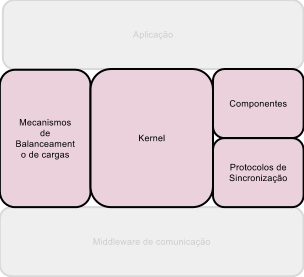
\includegraphics{camada_framework.png}}
  \caption{A camada aqui denominada \textit{framework}.}
\label{fig:camada_central}
\end{figure}

\section{O módulo Componente}

Um componente é uma abstração de um comportamento que desejamos reproduzir na nossa simulação. Na abstração de um sistema de caixa de supermercados, por exemplos, pode-se extrair três componentes (que são comuns em muitas situações na simulação de eventos discretos): o produtor, a fila de espera e o consumidor. O produtor seria o encarregado por criar clientes e envia-los à fila de espera para que o conumidor, que representa o caixa do supermercado, execute cada evento.

Uma biblioteca de componentes deve proporcionar objetos parametrizáveis que permitam a descrição do comportamento de cada um deles. No caso citado anteriormente, o componete produtor deve suportar parâmetros que, por exemplo, descreva a taxa de criação de novos evento, e as características de cada evento criado.

Os componentes são construidos diretamente em cima do objeto \textit{process} da camada de comunicação. Isso garante ao componente criado, por herança direta, toda funcionalidade de comunicação com outros componentes. Desta maneira, basta ao usuário do framework descrever na modelagem qual a conexão que cada componente faz, que esta é reproduzida automaticamente pelo framework, independente se esses componentes são processo cohabitantes ou não-cohabitantes.

Em alguns casos é conveniente que componentes sejam combinados a fim de que um novo componente seja criado. Uma das justificativas seria, por exemplo, garantir que dois componentes primitivos se comportem como um único compoente, evitando assim que estes sejam por ventura separados e passem a cohabitar ambientes diferentes. 

Em um exemplo, é conveniente que o um componente do tipo fila, que tem como características armazenar eventos que serão consumidos por um componente do tipo consumidor, seja encapsulado junto ao seu consumidor, evitando assim a possibilidade de que estes se separem, e diminuindo a quantidade de mensagens que trafegariam pela rede.

\section{Componentes básicos}

O tipo primitivo de um componente no \textit{framework} proposto é desenvolvido em cima da classe \textit{process} (conforme ilustrado na figura~\ref{fig:basic_component}) e deve ser capaz de proporcionar alguns elementos básicos para o controle do fluxo de eventos, como por exemplo um (ou diversos) canais de entrada de eventos, ambiente de processamento e canais de saída de eventos.

Sobre este componente primitivo são construídos quatro componentes básicos(Figura~\ref{fig:uml_components}), suficientes para demonstrar a implementação de alguns modelos para simulação. Estes componentes são: fila, gerador, consumidor e divisor.

\begin{figure}
  \centerline{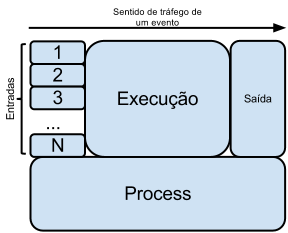
\includegraphics{basic_component.png}}
  \caption{Arquitetura básica de um componente primitivo.}
\label{fig:basic_component}
\end{figure}

\begin{figure}
  \centerline{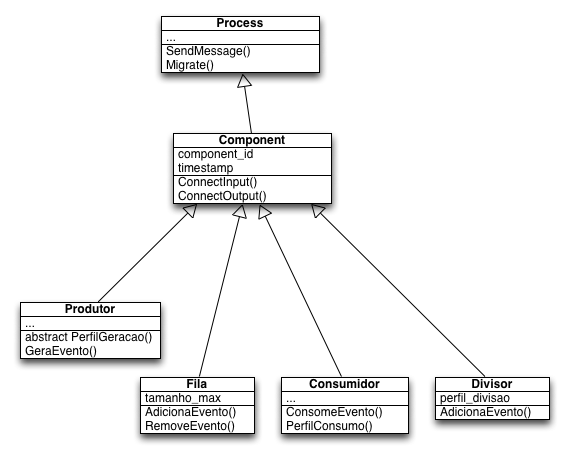
\includegraphics{uml_componentes.png}}
  \caption{Hierarquia dos componentes básicos.}
\label{fig:uml_components}
\end{figure}


Por motivos naturais, nem todos os componentes implementos esse modelo em sua totalidade. Componentes como os geradores de eventos, por exemplo, não possuem canais de entrada de eventos, uma vez que a sua função é a de apenas gerar novos eventos com base em uma parametrização de suas características para que se comporte conforme o modelo que descreve suas ações. 

\subsection{O componente Fila}

A fila é o componente responsável por armazenar eventos, ordenando-os com base no seu \textit{timestamp}. Cada evento que chega à fila é alocado respeitando a ordem referente ao seu \textit{timestamp}, e cada vez que um elemento é retirado da fila, isto é feito retirando-se o primeiro elemento da fila, ou seja, o elemento com o menor \textit{timestamp}. 

A fila é um componente passivo, ou seja, ela não executa nenhum tipo de ação sobre os eventos nela existente. Por ser um componente passivo, é o componente gerador que deve executar a ação de inserir um novo evento na fila, e é um componente consumidor que deve executar a ação de retirar o evento de menor \textit{timestamp} da fila.

Uma das características mais importantes do componente fila é o seu tamanho. Uma fila pode ou não ter um tamanho definido, porém uma vez definido um tamanho para esta fila, quando este tamanho se excede, ou seja, quando a quantidade de eventos inseridos cresce em uma velocidade tão grande que o consumidor atrelado àquela fila não consegue consumi-los em tempo hábil podem ocorrer dois eventos, dependendo de como o usuário do framework descreveu em seu modelo. No caso mais simples o usuário determina que ao se exceder a quantidade de elementos em uma fila, uma excessão do tipo QueueOverflow() seja lançada, e a simulação se encerra.

Em um caso mais elaborado, ao se atingir o limite de uma fila esta pode apenas negar a inserção de novos elementos até que haja espaço suficiente. Neste caso, há uma propagação da condição de estacionamento da execução para os elementos atrelados à essa fila, causando um efeito que reflete em grande parte do sistema. 

\begin{figure}
  \centerline{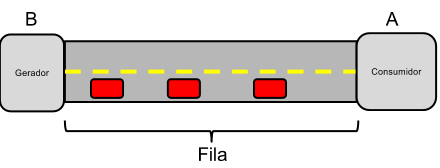
\includegraphics{cruzamento.png}}
  \caption{Modelagem de uma via urbana.}
\label{fig:cruzamento}
\end{figure}

Um exemplo típico que ilustra esse caso é a simulação de uma sequência de cruzamentos em uma via urbana, ilustrada na Figura~\ref{fig:cruzamento}. A quantidade de carros que cabem em um intervalo entre os dois cruzamentos A e B é finito, e se o cruzamento A não consome carros em uma velocidade maior ou igual à que eles chegam, há um crescimento na quantidade de carros entre os dois cruzamentos, o que pode levar à paralização temporária da simulação, até que o consumidor A consuma eventos, liberando espaço na fila.

\subsection{O componente Gerador}

Assim como ilustrado na Figura~\ref{fig:cruzamento}, um exemplo de gerador de eventos é uma extremidade de uma via de trânsito, que gera eventos (no exemplo citado, carros) em uma determinada taxa de tempo, com uma determinada frequência.

Um dos comportamentos parametrizáveis do componente gerador é a função que modela a taxa de criação de novos eventos ao longo do tempo. Um sistema que se deseja maior fidelidade quanto aos dados simulados deve permitir uma detalhada parametrização do comportamento de seus componentes. Neste \textit{framework} isto é feito através das funções geradoras, que são funções que recebem como parâmetros dados da simulação e resultam em decisões sobre a criação ou não de novos eventos, e o comportamento desses eventos.

Mais detalhes sobre o funcionamento das funções geradoras são abordados na seção~\ref{funcoes_geradoras}.

\subsection{O componente Consumidor}

Assim como o componente gerador, o componente consumidor é parametrizável através de funções externas que descrevem o seu comportamento ao longo do tempo de simulação. Outros dados levados em conta durante a execução de um evento por um consumidor são as características internas dos eventos.

O componente gerador possui múltiplas entradas de dados, porém apenas um canal de saída. Uma saída do gerador pode ser dividida em várias utilizando um componente divisor(ver subseção~\ref{divisor}). A razão de se adotar este \textit{design} de um único canal de saída e múltiplas entradas se justifica pela simplicidade da arquitetura do modelo, uma vez que o componente gerador não precisaria se encarregar do comportamento que os eventos por ele processados tomariam após o processamento.

\begin{figure}
  \centerline{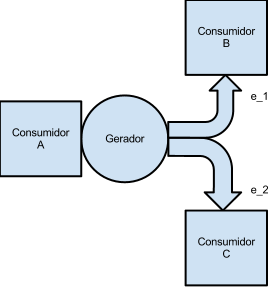
\includegraphics{gerador_mais_consumidor.png}}
  \caption{Um processo consumidor que gera eventos. No caso ilustrado, o consumidor A gera, através de um componente Gerador, simultaneamente os eventos e\_1 e e\_2 que são então encaminhados para os consumidores B e C}
\label{fig:multiple_sons}
\end{figure}

Uma vez que o evento é processado por um consumidor, este pode tomar três caminhos distintos: o evento pode simplesmente morrer, o evento pode ser redirecionado para um novo processador (ou mesmo para o mesmo processador, dependendo da necessidade da simulação), porém com suas características originais mantidas. Uma terceira possibilidade é que o evento sofra uma modificação nas suas características antes de ser encaminhado a diante.

Em condições especiais, um componente processador pode ser conectado à um gerador, e a ação de executar um evento poderia gerar um ou mais eventos distintos por esse gerador, que seriam então inseridos no sistema. Um exemplo prático desta aplicação é a simulação do fluxo de trabalho de uma companhia, onde a chegada de um documento pode disparar duas tarefas diferentes a serem feitas em paralelo (Figura~\ref{fig:multiple_sons}).


\subsection{O componente Divisor \label{divisor}}

Um componente divisor possui multiplas entradas e múltiplos canais de saída. A sua função é, dado um evento e que entra pelo divisor, aplicar uma função de decisão que mapeie este evnto para uma de suas saídas.

Assim como os componentes consumidor e gerador, o comportamento de um divisor é parametrizável através de funções que descrevem o seu comportamento com base nas características do modelo simulado.

A aplicação mais comum de um divisor é atrelado à saída de um processador, ou de um gerador, a fim de o evento que é entregue a ele seja redirecionado a um caminho aleatório, porém descrito por sua função de comportamento.

\section{O \textit{kernel} do \textit{framework}}

A parte central do \textit{framework} desenvolvido neste trabalho aqui é ilustrada pelo módulo \textit{kernel} (Figura~\ref{fig:camada_central}). O \textit{kernel} é o responsável por gerenciar a simulação, incrementando o \textit{timestep} de cada componente, e tomando decisões de migração, comunicação, sincronismo e balanceamento de carga.

Para realizar tais funções o kernel se apoia diretamente no \textit{middleware} de comunicação descrito no capítulo~\ref{chapter_middleware}, além de utilizar os algorítmos de balanceamento de carga e os protocolos de sincronismo da simulação.

A cada incremento discreto da simulação, denominado \textit{timestep}, o kernel do \textit{framework} realiza as seguintes funções:

\begin{itemize}
\item Incrementar o \textit{timestamp} de cada componente.
\item Verificar se existem mensagens no \textit{buffer} do middleware, e tentar redireciona-las ao destinatário.
\item Verificar, através do módulo de balanceamento de cargas, se existem processos que devem ser migrados.
\item Verificar, através do módulo de sincronismo, se ocorreram mensagens \textit{straggler}. Caso afirmativo, designa ao módulo de sincronismo a tarefa de re-sincronizar o sistema.
\item Gerencia, através do módulo de sincronismo, as tarefas de salvamento de estados.
\end{itemize}

O \textit{kernel} do sistema executa estes processos em \textit{loop} até que o números de iterações previstas acabe, ou até que a simulação seja interrompida por algum evento externo.

\section{Protocolos de sincronização}

Uma das premissas do projeto é a possibilidade de se substituir certos módulos do framework conforme a necessidade do seu usuário. Este encapsulamento de certas funcionalidades do \textit{framework} possibilita uma facilidade quando se deseja trocar algum componente do sistema.

Para que isto seja possível, o \textit{kernel} do sistema deve garantir uma \textit{interface} de acessos a diveras funções e variáveis do ambiente, permitindo assim que o módulo adquira dados referentes à simulação e interfira no seu funcionamento.

No caso da sincronização dos processos, o módulo em questão deve ser capaz de adquirir valores como o \textit{LVT} e o \textit{GVT}, idendtificar mensagens \textit{straggler}, além de ter acesso ao \textit{middleware} de comunicação para trocar mensagens com os demais nós do sistemas, e requerer o \textit{rollback} para um determinado \textit{timestamp}.

\section{Algoritmos de balanceamento de carga}

Assim como no caso dos protocolos de sincronização de eventos, os algorítmos de balanceamento de cargas do sistema também são modularidos e podem ser trocados pelo usuário (ou até mesmo customizados).

Cabe ao \textit{framework} prover uma interface que possibilite ao módulo de balanceamento requerere ao \textit{kernel} informações sobre a carga de cada nó do sistema, tal qual o perfil de comunicação de cada \textit{process}. Com base nesses dados, o algorítmo decide qual processo deve ser migrado, e para qual máquina.

Para que a migração seja possível, o \textit{kernel} deve prover mecanismos para que o módulo de balanceamento de cargas requira a migração de um determinado processo.
